\documentclass[1p]{elsarticle_modified}
%\bibliographystyle{elsarticle-num}

%\usepackage[colorlinks]{hyperref}
%\usepackage{abbrmath_seonhwa} %\Abb, \Ascr, \Acal ,\Abf, \Afrak
\usepackage{amsfonts}
\usepackage{amssymb}
\usepackage{amsmath}
\usepackage{amsthm}
\usepackage{scalefnt}
\usepackage{amsbsy}
\usepackage{kotex}
\usepackage{caption}
\usepackage{subfig}
\usepackage{color}
\usepackage{graphicx}
\usepackage{xcolor} %% white, black, red, green, blue, cyan, magenta, yellow
\usepackage{float}
\usepackage{setspace}
\usepackage{hyperref}

\usepackage{tikz}
\usetikzlibrary{arrows}

\usepackage{multirow}
\usepackage{array} % fixed length table
\usepackage{hhline}

%%%%%%%%%%%%%%%%%%%%%
\makeatletter
\renewcommand*\env@matrix[1][\arraystretch]{%
	\edef\arraystretch{#1}%
	\hskip -\arraycolsep
	\let\@ifnextchar\new@ifnextchar
	\array{*\c@MaxMatrixCols c}}
\makeatother %https://tex.stackexchange.com/questions/14071/how-can-i-increase-the-line-spacing-in-a-matrix
%%%%%%%%%%%%%%%

\usepackage[normalem]{ulem}

\newcommand{\msout}[1]{\ifmmode\text{\sout{\ensuremath{#1}}}\else\sout{#1}\fi}
%SOURCE: \msout is \stkout macro in https://tex.stackexchange.com/questions/20609/strikeout-in-math-mode

\newcommand{\cancel}[1]{
	\ifmmode
	{\color{red}\msout{#1}}
	\else
	{\color{red}\sout{#1}}
	\fi
}

\newcommand{\add}[1]{
	{\color{blue}\uwave{#1}}
}

\newcommand{\replace}[2]{
	\ifmmode
	{\color{red}\msout{#1}}{\color{blue}\uwave{#2}}
	\else
	{\color{red}\sout{#1}}{\color{blue}\uwave{#2}}
	\fi
}

\newcommand{\Sol}{\mathcal{S}} %segment
\newcommand{\D}{D} %diagram
\newcommand{\A}{\mathcal{A}} %arc


%%%%%%%%%%%%%%%%%%%%%%%%%%%%%5 test

\def\sl{\operatorname{\textup{SL}}(2,\Cbb)}
\def\psl{\operatorname{\textup{PSL}}(2,\Cbb)}
\def\quan{\mkern 1mu \triangleright \mkern 1mu}

\theoremstyle{definition}
\newtheorem{thm}{Theorem}[section]
\newtheorem{prop}[thm]{Proposition}
\newtheorem{lem}[thm]{Lemma}
\newtheorem{ques}[thm]{Question}
\newtheorem{cor}[thm]{Corollary}
\newtheorem{defn}[thm]{Definition}
\newtheorem{exam}[thm]{Example}
\newtheorem{rmk}[thm]{Remark}
\newtheorem{alg}[thm]{Algorithm}

\newcommand{\I}{\sqrt{-1}}
\begin{document}

%\begin{frontmatter}
%
%\title{Boundary parabolic representations of knots up to 8 crossings}
%
%%% Group authors per affiliation:
%\author{Yunhi Cho} 
%\address{Department of Mathematics, University of Seoul, Seoul, Korea}
%\ead{yhcho@uos.ac.kr}
%
%
%\author{Seonhwa Kim} %\fnref{s_kim}}
%\address{Center for Geometry and Physics, Institute for Basic Science, Pohang, 37673, Korea}
%\ead{ryeona17@ibs.re.kr}
%
%\author{Hyuk Kim}
%\address{Department of Mathematical Sciences, Seoul National University, Seoul 08826, Korea}
%\ead{hyukkim@snu.ac.kr}
%
%\author{Seokbeom Yoon}
%\address{Department of Mathematical Sciences, Seoul National University, Seoul, 08826,  Korea}
%\ead{sbyoon15@snu.ac.kr}
%
%\begin{abstract}
%We find all boundary parabolic representation of knots up to 8 crossings.
%
%\end{abstract}
%\begin{keyword}
%    \MSC[2010] 57M25 
%\end{keyword}
%
%\end{frontmatter}

%\linenumbers
%\tableofcontents
%
\newcommand\colored[1]{\textcolor{white}{\rule[-0.35ex]{0.8em}{1.4ex}}\kern-0.8em\color{red} #1}%
%\newcommand\colored[1]{\textcolor{white}{ #1}\kern-2.17ex	\textcolor{white}{ #1}\kern-1.81ex	\textcolor{white}{ #1}\kern-2.15ex\color{red}#1	}

{\Large $\underline{11a_{357}~(K11a_{357})}$}

\setlength{\tabcolsep}{10pt}
\renewcommand{\arraystretch}{1.6}
\vspace{1cm}\begin{tabular}{m{100pt}>{\centering\arraybackslash}m{274pt}}
\multirow{5}{120pt}{
	\centering
	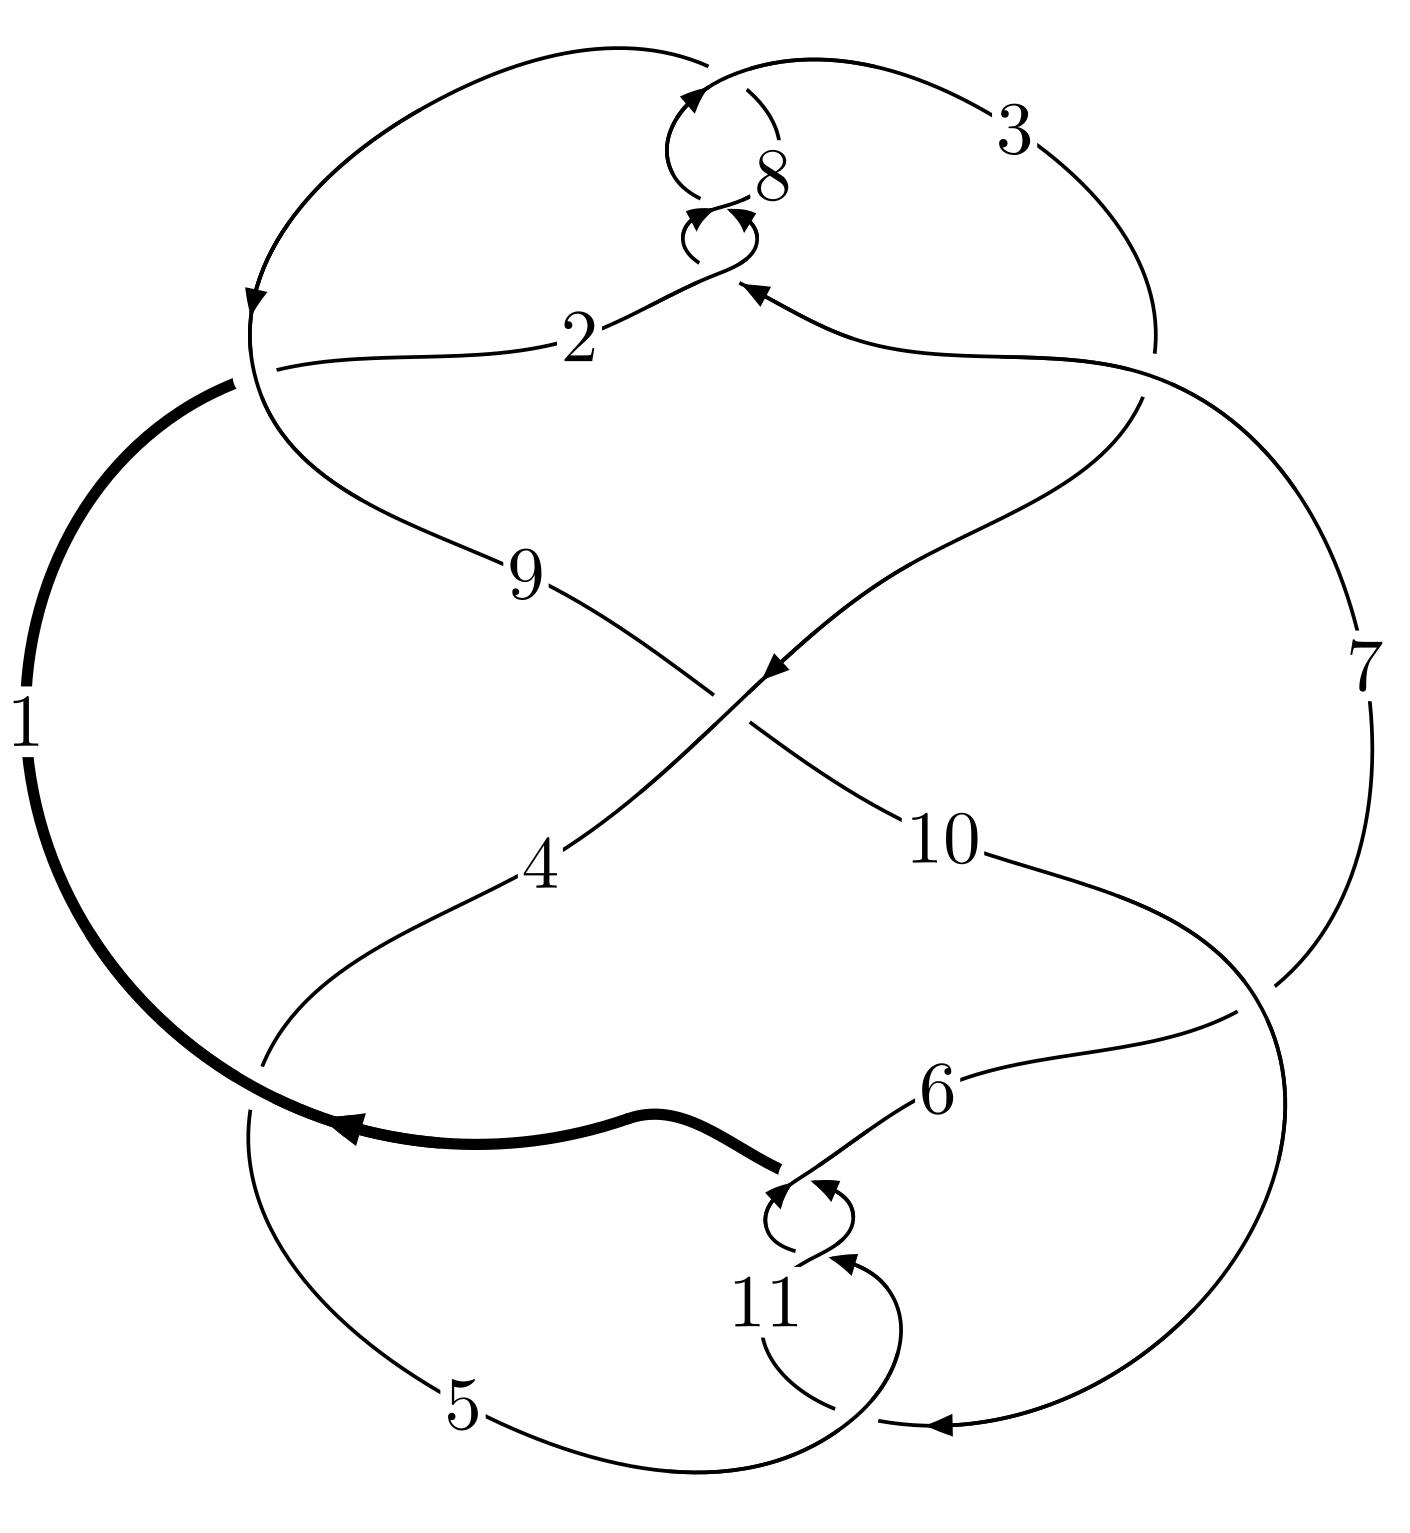
\includegraphics[width=112pt]{../../../GIT/diagram.site/Diagrams/png/606_11a_357.png}\\
\ \ \ A knot diagram\footnotemark}&
\allowdisplaybreaks
\textbf{Linearized knot diagam} \\
\cline{2-2}
 &
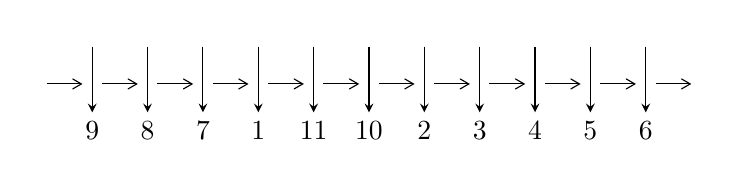
\begin{tikzpicture}[x=20pt, y=17pt]
	% nodes
	\node (C0) at (0, 0) {};
	\node (C1) at (1, 0) {};
	\node (C1U) at (1, +1) {};
	\node (C1D) at (1, -1) {9};

	\node (C2) at (2, 0) {};
	\node (C2U) at (2, +1) {};
	\node (C2D) at (2, -1) {8};

	\node (C3) at (3, 0) {};
	\node (C3U) at (3, +1) {};
	\node (C3D) at (3, -1) {7};

	\node (C4) at (4, 0) {};
	\node (C4U) at (4, +1) {};
	\node (C4D) at (4, -1) {1};

	\node (C5) at (5, 0) {};
	\node (C5U) at (5, +1) {};
	\node (C5D) at (5, -1) {11};

	\node (C6) at (6, 0) {};
	\node (C6U) at (6, +1) {};
	\node (C6D) at (6, -1) {10};

	\node (C7) at (7, 0) {};
	\node (C7U) at (7, +1) {};
	\node (C7D) at (7, -1) {2};

	\node (C8) at (8, 0) {};
	\node (C8U) at (8, +1) {};
	\node (C8D) at (8, -1) {3};

	\node (C9) at (9, 0) {};
	\node (C9U) at (9, +1) {};
	\node (C9D) at (9, -1) {4};

	\node (C10) at (10, 0) {};
	\node (C10U) at (10, +1) {};
	\node (C10D) at (10, -1) {5};

	\node (C11) at (11, 0) {};
	\node (C11U) at (11, +1) {};
	\node (C11D) at (11, -1) {6};
	\node (C12) at (12, 0) {};

	% arrows
	\draw[->,>={angle 60}]
	(C0) edge (C1) (C1) edge (C2) (C2) edge (C3) (C3) edge (C4) (C4) edge (C5) (C5) edge (C6) (C6) edge (C7) (C7) edge (C8) (C8) edge (C9) (C9) edge (C10) (C10) edge (C11) (C11) edge (C12) ;	\draw[->,>=stealth]
	(C1U) edge (C1D) (C2U) edge (C2D) (C3U) edge (C3D) (C4U) edge (C4D) (C5U) edge (C5D) (C6U) edge (C6D) (C7U) edge (C7D) (C8U) edge (C8D) (C9U) edge (C9D) (C10U) edge (C10D) (C11U) edge (C11D) ;
	\end{tikzpicture} \\
\hhline{~~} \\& 
\textbf{Solving Sequence} \\ \cline{2-2} 
 &
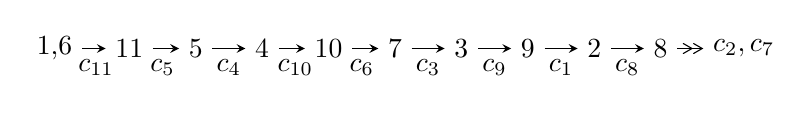
\begin{tikzpicture}[x=24pt, y=7pt]
	% node
	\node (A0) at (-1/8, 0) {1,6};
	\node (A1) at (1, 0) {11};
	\node (A2) at (2, 0) {5};
	\node (A3) at (3, 0) {4};
	\node (A4) at (4, 0) {10};
	\node (A5) at (5, 0) {7};
	\node (A6) at (6, 0) {3};
	\node (A7) at (7, 0) {9};
	\node (A8) at (8, 0) {2};
	\node (A9) at (9, 0) {8};
	\node (C1) at (1/2, -1) {$c_{11}$};
	\node (C2) at (3/2, -1) {$c_{5}$};
	\node (C3) at (5/2, -1) {$c_{4}$};
	\node (C4) at (7/2, -1) {$c_{10}$};
	\node (C5) at (9/2, -1) {$c_{6}$};
	\node (C6) at (11/2, -1) {$c_{3}$};
	\node (C7) at (13/2, -1) {$c_{9}$};
	\node (C8) at (15/2, -1) {$c_{1}$};
	\node (C9) at (17/2, -1) {$c_{8}$};
	\node (A10) at (41/4, 0) {$c_{2},c_{7}$};

	% edge
	\draw[->,>=stealth]	
	(A0) edge (A1) (A1) edge (A2) (A2) edge (A3) (A3) edge (A4) (A4) edge (A5) (A5) edge (A6) (A6) edge (A7) (A7) edge (A8) (A8) edge (A9) ;
	\draw[->>,>={angle 60}]	
	(A9) edge (A10);
\end{tikzpicture} \\ 

\end{tabular} \\

\footnotetext{
The image of knot diagram is generated by the software ``\textbf{Draw programme}" developed by Andrew Bartholomew(\url{http://www.layer8.co.uk/maths/draw/index.htm\#Running-draw}), where we modified some parts for our purpose(\url{https://github.com/CATsTAILs/LinksPainter}).
}\phantom \\ \newline 
\centering \textbf{Ideals for irreducible components\footnotemark of $X_{\text{par}}$} 
 
\begin{align*}
I^u_{1}&=\langle 
u^9-4 u^7+5 u^5+u^2-3 u-1\rangle \\
I^u_{2}&=\langle 
u^{36}- u^{35}+\cdots-4 u^3+1\rangle \\
\\
\end{align*}
\raggedright * 2 irreducible components of $\dim_{\mathbb{C}}=0$, with total 45 representations.\\
\footnotetext{All coefficients of polynomials are rational numbers. But the coefficients are sometimes approximated in decimal forms when there is not enough margin.}
\newpage
\renewcommand{\arraystretch}{1}
\centering \section*{I. $I^u_{1}= \langle u^9-4 u^7+5 u^5+u^2-3 u-1 \rangle$}
\flushleft \textbf{(i) Arc colorings}\\
\begin{tabular}{m{7pt} m{180pt} m{7pt} m{180pt} }
\flushright $a_{1}=$&$\begin{pmatrix}1\\0\end{pmatrix}$ \\
\flushright $a_{6}=$&$\begin{pmatrix}0\\u\end{pmatrix}$ \\
\flushright $a_{11}=$&$\begin{pmatrix}1\\- u^2\end{pmatrix}$ \\
\flushright $a_{5}=$&$\begin{pmatrix}u\\- u^3+u\end{pmatrix}$ \\
\flushright $a_{4}=$&$\begin{pmatrix}- u^3+2 u\\- u^3+u\end{pmatrix}$ \\
\flushright $a_{10}=$&$\begin{pmatrix}- u^2+1\\u^4-2 u^2\end{pmatrix}$ \\
\flushright $a_{7}=$&$\begin{pmatrix}- u^5+2 u^3- u\\u^7-3 u^5+2 u^3+u\end{pmatrix}$ \\
\flushright $a_{3}=$&$\begin{pmatrix}u^8-3 u^6+3 u^4- u^3- u^2+2 u\\u^4-2 u^2\end{pmatrix}$ \\
\flushright $a_{9}=$&$\begin{pmatrix}- u^8+3 u^6-3 u^4- u^3+u+1\\- u^3+u\end{pmatrix}$ \\
\flushright $a_{2}=$&$\begin{pmatrix}u^7+u^6-3 u^5-3 u^4+2 u^3+2 u^2+u+1\\u^6-2 u^4+u^2\end{pmatrix}$ \\
\flushright $a_{8}=$&$\begin{pmatrix}- u^8- u^7+3 u^6+2 u^5-2 u^4- u^2-2 u\\- u^5+u^3+u\end{pmatrix}$\\ \flushright $a_{8}=$&$\begin{pmatrix}- u^8- u^7+3 u^6+2 u^5-2 u^4- u^2-2 u\\- u^5+u^3+u\end{pmatrix}$\\&\end{tabular}
\flushleft \textbf{(ii) Obstruction class $= -1$}\\~\\
\flushleft \textbf{(iii) Cusp Shapes $= -4 u^6+4 u^5+12 u^4-8 u^3-8 u^2+4 u-18$}\\~\\
\newpage\renewcommand{\arraystretch}{1}
\flushleft \textbf{(iv) u-Polynomials at the component}\newline \\
\begin{tabular}{m{50pt}|m{274pt}}
Crossings & \hspace{64pt}u-Polynomials at each crossing \\
\hline $$\begin{aligned}c_{1},c_{3},c_{4}\\c_{6}\end{aligned}$$&$\begin{aligned}
&u^9+4 u^7-2 u^6+5 u^5-6 u^4-2 u^3-5 u^2-5 u-1
\end{aligned}$\\
\hline $$\begin{aligned}c_{2},c_{5},c_{7}\\c_{8},c_{10},c_{11}\end{aligned}$$&$\begin{aligned}
&u^9-4 u^7+5 u^5+u^2-3 u-1
\end{aligned}$\\
\hline $$\begin{aligned}c_{9}\end{aligned}$$&$\begin{aligned}
&u^9+7 u^8+25 u^7+54 u^6+74 u^5+55 u^4+u^3-42 u^2-36 u-8
\end{aligned}$\\
\hline
\end{tabular}\\~\\
\newpage\renewcommand{\arraystretch}{1}
\flushleft \textbf{(v) Riley Polynomials at the component}\newline \\
\begin{tabular}{m{50pt}|m{274pt}}
Crossings & \hspace{64pt}Riley Polynomials at each crossing \\
\hline $$\begin{aligned}c_{1},c_{3},c_{4}\\c_{6}\end{aligned}$$&$\begin{aligned}
&y^9+8 y^8+26 y^7+32 y^6-25 y^5-116 y^4-110 y^3-17 y^2+15 y-1
\end{aligned}$\\
\hline $$\begin{aligned}c_{2},c_{5},c_{7}\\c_{8},c_{10},c_{11}\end{aligned}$$&$\begin{aligned}
&y^9-8 y^8+26 y^7-40 y^6+19 y^5+24 y^4-30 y^3- y^2+11 y-1
\end{aligned}$\\
\hline $$\begin{aligned}c_{9}\end{aligned}$$&$\begin{aligned}
&y^9+y^8+17 y^7+16 y^6+102 y^5-29 y^4+157 y^3-956 y^2+624 y-64
\end{aligned}$\\
\hline
\end{tabular}\\~\\
\newpage\flushleft \textbf{(vi) Complex Volumes and Cusp Shapes}
$$\begin{array}{c|c|c}  
\text{Solutions to }I^u_{1}& \I (\text{vol} + \sqrt{-1}CS) & \text{Cusp shape}\\
 \hline 
\begin{aligned}
u &= \phantom{-}0.098375 + 0.814801 I\end{aligned}
 & \phantom{-}7.35406 - 4.61617 I & -4.22495 + 4.01969 I \\ \hline\begin{aligned}
u &= \phantom{-}0.098375 - 0.814801 I\end{aligned}
 & \phantom{-}7.35406 + 4.61617 I & -4.22495 - 4.01969 I \\ \hline\begin{aligned}
u &= \phantom{-}1.18251\phantom{ +0.000000I}\end{aligned}
 & -5.71950\phantom{ +0.000000I} & -15.9090\phantom{ +0.000000I} \\ \hline\begin{aligned}
u &= -1.188580 + 0.361061 I\end{aligned}
 & \phantom{-}0.69960 + 3.87858 I & -10.64109 - 3.78555 I \\ \hline\begin{aligned}
u &= -1.188580 - 0.361061 I\end{aligned}
 & \phantom{-}0.69960 - 3.87858 I & -10.64109 + 3.78555 I \\ \hline\begin{aligned}
u &= -1.37937\phantom{ +0.000000I}\end{aligned}
 & -11.3909\phantom{ +0.000000I} & -21.8270\phantom{ +0.000000I} \\ \hline\begin{aligned}
u &= \phantom{-}1.341750 + 0.354713 I\end{aligned}
 & -1.71371 - 13.05000 I & -13.4391 + 8.3124 I \\ \hline\begin{aligned}
u &= \phantom{-}1.341750 - 0.354713 I\end{aligned}
 & -1.71371 + 13.05000 I & -13.4391 - 8.3124 I \\ \hline\begin{aligned}
u &= -0.306233\phantom{ +0.000000I}\end{aligned}
 & -0.504287\phantom{ +0.000000I} & -19.6540\phantom{ +0.000000I}\\
 \hline 
 \end{array}$$\newpage\newpage\renewcommand{\arraystretch}{1}
\centering \section*{II. $I^u_{2}= \langle u^{36}- u^{35}+\cdots-4 u^3+1 \rangle$}
\flushleft \textbf{(i) Arc colorings}\\
\begin{tabular}{m{7pt} m{180pt} m{7pt} m{180pt} }
\flushright $a_{1}=$&$\begin{pmatrix}1\\0\end{pmatrix}$ \\
\flushright $a_{6}=$&$\begin{pmatrix}0\\u\end{pmatrix}$ \\
\flushright $a_{11}=$&$\begin{pmatrix}1\\- u^2\end{pmatrix}$ \\
\flushright $a_{5}=$&$\begin{pmatrix}u\\- u^3+u\end{pmatrix}$ \\
\flushright $a_{4}=$&$\begin{pmatrix}- u^3+2 u\\- u^3+u\end{pmatrix}$ \\
\flushright $a_{10}=$&$\begin{pmatrix}- u^2+1\\u^4-2 u^2\end{pmatrix}$ \\
\flushright $a_{7}=$&$\begin{pmatrix}- u^5+2 u^3- u\\u^7-3 u^5+2 u^3+u\end{pmatrix}$ \\
\flushright $a_{3}=$&$\begin{pmatrix}- u^{15}+6 u^{13}-14 u^{11}+14 u^9-2 u^7-6 u^5+2 u^3+2 u\\u^{17}-7 u^{15}+19 u^{13}-22 u^{11}+3 u^9+14 u^7-6 u^5-4 u^3+u\end{pmatrix}$ \\
\flushright $a_{9}=$&$\begin{pmatrix}u^{10}-5 u^8+8 u^6-3 u^4-3 u^2+1\\u^{10}-4 u^8+5 u^6-3 u^2\end{pmatrix}$ \\
\flushright $a_{2}=$&$\begin{pmatrix}u^{20}-9 u^{18}+\cdots-3 u^2+1\\u^{20}-8 u^{18}+26 u^{16}-40 u^{14}+19 u^{12}+24 u^{10}-30 u^8+9 u^4\end{pmatrix}$ \\
\flushright $a_{8}=$&$\begin{pmatrix}2 u^{35}- u^{34}+\cdots-7 u^2+1\\- u^{34}+14 u^{32}+\cdots-4 u^2+3 u\end{pmatrix}$\\ \flushright $a_{8}=$&$\begin{pmatrix}2 u^{35}- u^{34}+\cdots-7 u^2+1\\- u^{34}+14 u^{32}+\cdots-4 u^2+3 u\end{pmatrix}$\\&\end{tabular}
\flushleft \textbf{(ii) Obstruction class $= -1$}\\~\\
\flushleft \textbf{(iii) Cusp Shapes $= -4 u^{27}+44 u^{25}+4 u^{24}-208 u^{23}-40 u^{22}+532 u^{21}+172 u^{20}-732 u^{19}-400 u^{18}+348 u^{17}+504 u^{16}+416 u^{15}-244 u^{14}-628 u^{13}-156 u^{12}+112 u^{11}+224 u^{10}+208 u^9-20 u^8-40 u^7-56 u^6-48 u^5+4 u^4-8 u^3+4 u^2-4 u-10$}\\~\\
\newpage\renewcommand{\arraystretch}{1}
\flushleft \textbf{(iv) u-Polynomials at the component}\newline \\
\begin{tabular}{m{50pt}|m{274pt}}
Crossings & \hspace{64pt}u-Polynomials at each crossing \\
\hline $$\begin{aligned}c_{1},c_{3},c_{4}\\c_{6}\end{aligned}$$&$\begin{aligned}
&u^{36}+3 u^{35}+\cdots-12 u-7
\end{aligned}$\\
\hline $$\begin{aligned}c_{2},c_{5},c_{7}\\c_{8},c_{10},c_{11}\end{aligned}$$&$\begin{aligned}
&u^{36}- u^{35}+\cdots-4 u^3+1
\end{aligned}$\\
\hline $$\begin{aligned}c_{9}\end{aligned}$$&$\begin{aligned}
&(u^{18}-3 u^{17}+\cdots-7 u+1)^{2}
\end{aligned}$\\
\hline
\end{tabular}\\~\\
\newpage\renewcommand{\arraystretch}{1}
\flushleft \textbf{(v) Riley Polynomials at the component}\newline \\
\begin{tabular}{m{50pt}|m{274pt}}
Crossings & \hspace{64pt}Riley Polynomials at each crossing \\
\hline $$\begin{aligned}c_{1},c_{3},c_{4}\\c_{6}\end{aligned}$$&$\begin{aligned}
&y^{36}+23 y^{35}+\cdots-340 y+49
\end{aligned}$\\
\hline $$\begin{aligned}c_{2},c_{5},c_{7}\\c_{8},c_{10},c_{11}\end{aligned}$$&$\begin{aligned}
&y^{36}-29 y^{35}+\cdots+8 y^2+1
\end{aligned}$\\
\hline $$\begin{aligned}c_{9}\end{aligned}$$&$\begin{aligned}
&(y^{18}+3 y^{17}+\cdots-31 y+1)^{2}
\end{aligned}$\\
\hline
\end{tabular}\\~\\
\newpage\flushleft \textbf{(vi) Complex Volumes and Cusp Shapes}
$$\begin{array}{c|c|c}  
\text{Solutions to }I^u_{2}& \I (\text{vol} + \sqrt{-1}CS) & \text{Cusp shape}\\
 \hline 
\begin{aligned}
u &= -0.114880 + 0.814996 I\end{aligned}
 & \phantom{-}2.86466 + 8.83442 I & -8.85054 - 6.32425 I \\ \hline\begin{aligned}
u &= -0.114880 - 0.814996 I\end{aligned}
 & \phantom{-}2.86466 - 8.83442 I & -8.85054 + 6.32425 I \\ \hline\begin{aligned}
u &= -0.075687 + 0.812840 I\end{aligned}
 & \phantom{-}4.10849 + 0.36044 I & -7.24415 - 0.04898 I \\ \hline\begin{aligned}
u &= -0.075687 - 0.812840 I\end{aligned}
 & \phantom{-}4.10849 - 0.36044 I & -7.24415 + 0.04898 I \\ \hline\begin{aligned}
u &= -1.137600 + 0.360537 I\end{aligned}
 & -0.25332 - 4.56891 I & -11.76762 + 2.55639 I \\ \hline\begin{aligned}
u &= -1.137600 - 0.360537 I\end{aligned}
 & -0.25332 + 4.56891 I & -11.76762 - 2.55639 I \\ \hline\begin{aligned}
u &= \phantom{-}1.161330 + 0.360877 I\end{aligned}
 & \phantom{-}4.10849 + 0.36044 I & -7.24415 - 0.04898 I \\ \hline\begin{aligned}
u &= \phantom{-}1.161330 - 0.360877 I\end{aligned}
 & \phantom{-}4.10849 - 0.36044 I & -7.24415 + 0.04898 I \\ \hline\begin{aligned}
u &= -0.042366 + 0.732635 I\end{aligned}
 & \phantom{-}2.49914 + 1.48028 I & -7.39740 - 4.69129 I \\ \hline\begin{aligned}
u &= -0.042366 - 0.732635 I\end{aligned}
 & \phantom{-}2.49914 - 1.48028 I & -7.39740 + 4.69129 I \\ \hline\begin{aligned}
u &= \phantom{-}0.125186 + 0.707270 I\end{aligned}
 & -2.91493 - 2.96900 I & -12.88830 + 4.22200 I \\ \hline\begin{aligned}
u &= \phantom{-}0.125186 - 0.707270 I\end{aligned}
 & -2.91493 + 2.96900 I & -12.88830 - 4.22200 I \\ \hline\begin{aligned}
u &= -1.253710 + 0.284832 I\end{aligned}
 & -1.22218 + 2.17847 I & -11.24475 + 0.74332 I \\ \hline\begin{aligned}
u &= -1.253710 - 0.284832 I\end{aligned}
 & -1.22218 - 2.17847 I & -11.24475 - 0.74332 I \\ \hline\begin{aligned}
u &= \phantom{-}1.294410 + 0.195773 I\end{aligned}
 & -6.07645\phantom{ +0.000000I} & -17.0816 + 0. I\phantom{ +0.000000I} \\ \hline\begin{aligned}
u &= \phantom{-}1.294410 - 0.195773 I\end{aligned}
 & -6.07645\phantom{ +0.000000I} & -17.0816 + 0. I\phantom{ +0.000000I} \\ \hline\begin{aligned}
u &= \phantom{-}1.31676\phantom{ +0.000000I}\end{aligned}
 & -5.41700\phantom{ +0.000000I} & -18.3110\phantom{ +0.000000I} \\ \hline\begin{aligned}
u &= \phantom{-}1.299400 + 0.312670 I\end{aligned}
 & -1.69882 - 5.26707 I & -12.9078 + 7.0444 I \\ \hline\begin{aligned}
u &= \phantom{-}1.299400 - 0.312670 I\end{aligned}
 & -1.69882 + 5.26707 I & -12.9078 - 7.0444 I \\ \hline\begin{aligned}
u &= -1.347930 + 0.085501 I\end{aligned}
 & -2.91493 + 2.96900 I & -12.88830 - 4.22200 I \\ \hline\begin{aligned}
u &= -1.347930 - 0.085501 I\end{aligned}
 & -2.91493 - 2.96900 I & -12.88830 + 4.22200 I \\ \hline\begin{aligned}
u &= \phantom{-}1.317490 + 0.356084 I\end{aligned}
 & -0.25332 - 4.56891 I & -11.76762 + 2.55639 I \\ \hline\begin{aligned}
u &= \phantom{-}1.317490 - 0.356084 I\end{aligned}
 & -0.25332 + 4.56891 I & -11.76762 - 2.55639 I \\ \hline\begin{aligned}
u &= -1.335910 + 0.303663 I\end{aligned}
 & -7.50591 + 6.65729 I & -18.0029 - 5.6815 I \\ \hline\begin{aligned}
u &= -1.335910 - 0.303663 I\end{aligned}
 & -7.50591 - 6.65729 I & -18.0029 + 5.6815 I \\ \hline\begin{aligned}
u &= \phantom{-}0.629383\phantom{ +0.000000I}\end{aligned}
 & -5.41700\phantom{ +0.000000I} & -18.3110\phantom{ +0.000000I} \\ \hline\begin{aligned}
u &= -1.332130 + 0.356156 I\end{aligned}
 & \phantom{-}2.86466 + 8.83442 I & -8.85054 - 6.32425 I \\ \hline\begin{aligned}
u &= -1.332130 - 0.356156 I\end{aligned}
 & \phantom{-}2.86466 - 8.83442 I & -8.85054 + 6.32425 I \\ \hline\begin{aligned}
u &= \phantom{-}1.377060 + 0.080377 I\end{aligned}
 & -7.50591 - 6.65729 I & -18.0029 + 5.6815 I \\ \hline\begin{aligned}
u &= \phantom{-}1.377060 - 0.080377 I\end{aligned}
 & -7.50591 + 6.65729 I & -18.0029 - 5.6815 I\\
 \hline 
 \end{array}$$\newpage$$\begin{array}{c|c|c}  
\text{Solutions to }I^u_{2}& \I (\text{vol} + \sqrt{-1}CS) & \text{Cusp shape}\\
 \hline 
\begin{aligned}
u &= -0.488414 + 0.379131 I\end{aligned}
 & -1.69882 + 5.26707 I & -12.9078 - 7.0444 I \\ \hline\begin{aligned}
u &= -0.488414 - 0.379131 I\end{aligned}
 & -1.69882 - 5.26707 I & -12.9078 + 7.0444 I \\ \hline\begin{aligned}
u &= \phantom{-}0.410957 + 0.392187 I\end{aligned}
 & \phantom{-}2.49914 - 1.48028 I & -7.39740 + 4.69129 I \\ \hline\begin{aligned}
u &= \phantom{-}0.410957 - 0.392187 I\end{aligned}
 & \phantom{-}2.49914 + 1.48028 I & -7.39740 - 4.69129 I \\ \hline\begin{aligned}
u &= -0.330280 + 0.456150 I\end{aligned}
 & -1.22218 - 2.17847 I & -11.24475 - 0.74332 I \\ \hline\begin{aligned}
u &= -0.330280 - 0.456150 I\end{aligned}
 & -1.22218 + 2.17847 I & -11.24475 + 0.74332 I\\
 \hline 
 \end{array}$$\newpage
\newpage\renewcommand{\arraystretch}{1}
\centering \section*{ III. u-Polynomials}
\begin{tabular}{m{50pt}|m{274pt}}
Crossings & \hspace{64pt}u-Polynomials at each crossing \\
\hline $$\begin{aligned}c_{1},c_{3},c_{4}\\c_{6}\end{aligned}$$&$\begin{aligned}
&(u^9+4 u^7-2 u^6+5 u^5-6 u^4-2 u^3-5 u^2-5 u-1)\\
&\cdot(u^{36}+3 u^{35}+\cdots-12 u-7)
\end{aligned}$\\
\hline $$\begin{aligned}c_{2},c_{5},c_{7}\\c_{8},c_{10},c_{11}\end{aligned}$$&$\begin{aligned}
&(u^9-4 u^7+5 u^5+u^2-3 u-1)(u^{36}- u^{35}+\cdots-4 u^3+1)
\end{aligned}$\\
\hline $$\begin{aligned}c_{9}\end{aligned}$$&$\begin{aligned}
&(u^9+7 u^8+25 u^7+54 u^6+74 u^5+55 u^4+u^3-42 u^2-36 u-8)\\
&\cdot(u^{18}-3 u^{17}+\cdots-7 u+1)^{2}
\end{aligned}$\\
\hline
\end{tabular}\newpage\renewcommand{\arraystretch}{1}
\centering \section*{ IV. Riley Polynomials}
\begin{tabular}{m{50pt}|m{274pt}}
Crossings & \hspace{64pt}Riley Polynomials at each crossing \\
\hline $$\begin{aligned}c_{1},c_{3},c_{4}\\c_{6}\end{aligned}$$&$\begin{aligned}
&(y^9+8 y^8+26 y^7+32 y^6-25 y^5-116 y^4-110 y^3-17 y^2+15 y-1)\\
&\cdot(y^{36}+23 y^{35}+\cdots-340 y+49)
\end{aligned}$\\
\hline $$\begin{aligned}c_{2},c_{5},c_{7}\\c_{8},c_{10},c_{11}\end{aligned}$$&$\begin{aligned}
&(y^9-8 y^8+26 y^7-40 y^6+19 y^5+24 y^4-30 y^3- y^2+11 y-1)\\
&\cdot(y^{36}-29 y^{35}+\cdots+8 y^2+1)
\end{aligned}$\\
\hline $$\begin{aligned}c_{9}\end{aligned}$$&$\begin{aligned}
&(y^9+y^8+17 y^7+16 y^6+102 y^5-29 y^4+157 y^3-956 y^2+624 y-64)\\
&\cdot(y^{18}+3 y^{17}+\cdots-31 y+1)^{2}
\end{aligned}$\\
\hline
\end{tabular}
\vskip 2pc
\end{document}